\documentclass[conference]{IEEEtran}
\IEEEoverridecommandlockouts
% The preceding line is only needed to identify funding in the first footnote. If that is unneeded, please comment it out.
\usepackage{cite}
\usepackage{listings}
\usepackage{amsmath,amssymb,amsfonts}
\usepackage[ruled,vlined]{algorithm2e}
\usepackage{algorithmic}
\usepackage{setspace, caption}
\usepackage{graphicx}
\usepackage{textcomp}
\usepackage{xcolor}
\def\BibTeX{{\rm B\kern-.05em{\sc i\kern-.025em b}\kern-.08em
    T\kern-.1667em\lower.7ex\hbox{E}\kern-.125emX}}
\begin{document}

\title{Find the Pivot in Rotated Sorted array
\\
{\footnotesize {
IV semester - Bachelor’s of Technology in Information technology with specialization in Business Informatics,\\
Indian Institute of Information Technology Allahabad, India
}}
\thanks{}
}

\author{\IEEEauthorblockN{1\textsuperscript{st} Amanjeet Kumar}
\IEEEauthorblockA{\textit{IIB2019006} \\
iiB2019006@iiita.ac.in \\
Amanjeetk11}
\and
\IEEEauthorblockN{2\textsuperscript{nd} Aditya Raj}
\IEEEauthorblockA{\textit{IIB2019007} \\
iib2019007@iiita.ac.in \\
Adityahulk}
\and
\IEEEauthorblockN{3\textsuperscript{rd} Shyam Tayal}
\IEEEauthorblockA{\textit{IIB2019008} \\
iib2019008@iiita.ac.in \\
shyamTayal}
}


\maketitle

\begin{abstract}
In this paper, we are devising an algorithm to find the Rotation Count in Rotated (clockwise) Sorted array. This paper also analyzes the time and space complexity of the algorithms used and provides the most efficient approach to solve the given problem.
\end{abstract}
\bigskip
\begin{IEEEkeywords}
array, sorted, rotated, clockwise, time complexity, space complexity, Divide and Conquer
\end{IEEEkeywords}

\section{Introduction}
An array is a collection of items stored at contiguous memory locations. The binary search algorithm uses Divide And Conquer approach which can be divided in three parts -
Divide: This involves dividing the problem into some sub problem.
Conquer: Sub problem by calling recursively until sub problem solved.
Combine: The Sub problem Solved so that we will get find problem solution.
\section{Algorithm Design}
We have devised two algorithms to Find the Rotation Count in Rotated Sorted array.

The First algorithm uses linear search to find the index of minimum element. As we can notice that the number of rotations is equal to index of minimum element. It is a simple approach is to find minimum element and returns its index.

\bigskip

\begin{algorithm}[H]
\begin{lstlisting}
function findPivot(a[], size):
      j = 0
      loop i in range (0 to size-1):
          if i > 0 and a[i-1] > a[i]:
              return j
\end{lstlisting}

 \caption{Naive Algorithm (Linear Search) }
\end{algorithm}

\bigskip
The second algorithm uses divide and conquer approach. Here also we find the index of minimum element, but using Binary Search.
\newline The minimum element is the only element whose previous is greater than it.
\newline If there is no previous element, then there is no rotation (first element is minimum).
\newline We check this condition for middle element by comparing it with (mid)’th and (mid+1)’th elements.
\newline If the minimum element is not at the middle (neither mid nor mid + 1), then minimum element lies in either left half or right half.
\newline If middle element is smaller than last element, then the minimum element lies in left half
\newline Else minimum element lies in right half.
\bigskip


\bigskip

\begin{algorithm}[H]
\begin{lstlisting}
function findPivot(arr[], N):
    if arr[0] <= arr[N-1] :
        return 0

    start = 0 , end = N-1;
    while start <= end  :
        mid = start + (end - start)/2

        if arr[mid] > arr[mid+1] :
            return mid+1

        if arr[start] <= arr[mid] :
            start = mid + 1
        else
            end = mid - 1

    return start
\end{lstlisting}

 \caption{Eficient Algorithm(Divide and Conquer)}
\end{algorithm}
\bigskip
\newpage


\section{Algorithm Analysis}

\subsection{Time Complexity}
    \subsubsection{Algorithm 1}
        \begin{itemize}
            Best Case:  $ \Omega(n) $\\
            Average Case: $\Theta(n)$ \\
            Worst Case: O(n)\\
        \end{itemize}
    \subsubsection{Algorithm 2}
        \begin{itemize}
            Best Case:  $ \Omega(1$)\\
            Average Case: $ \Theta(log(n))$ \\
            Worst Case: O($log(n)$)\\
        \end{itemize}

\subsection{Space Complexity}
    \subsubsection{Algorithm 1}
        \begin{itemize}
            O(1)\\
        \end{itemize}
    \subsubsection{Algorithm 2}
        \begin{itemize}
            O(1)\\
        \end{itemize}

Random number generator has been used for filling the arrays in every case.
Following graphs compare the times taken by the Linear Search as well as Divide and Conquer approaches.
% \newpage


\begin{figure}[h!]
\centerline{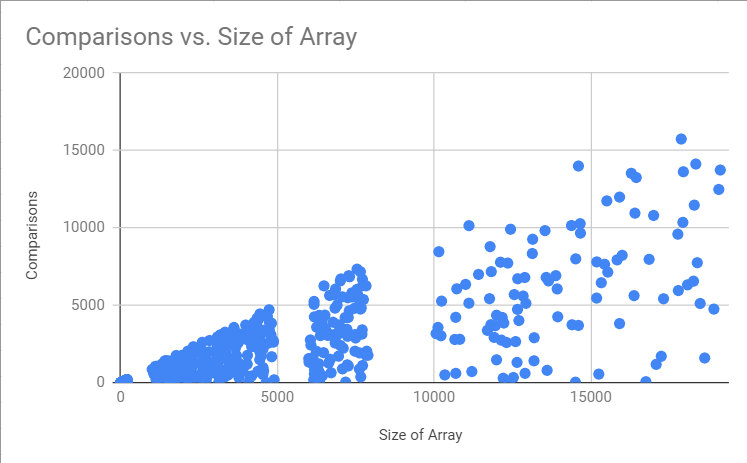
\includegraphics[width=80mm]{tc_naive.png}}
\caption{Algorithm 1 VS N}
\centerline{\textit{ }}
\label{fig:graph}
\end{figure}

\begin{figure}[h!]
\centerline{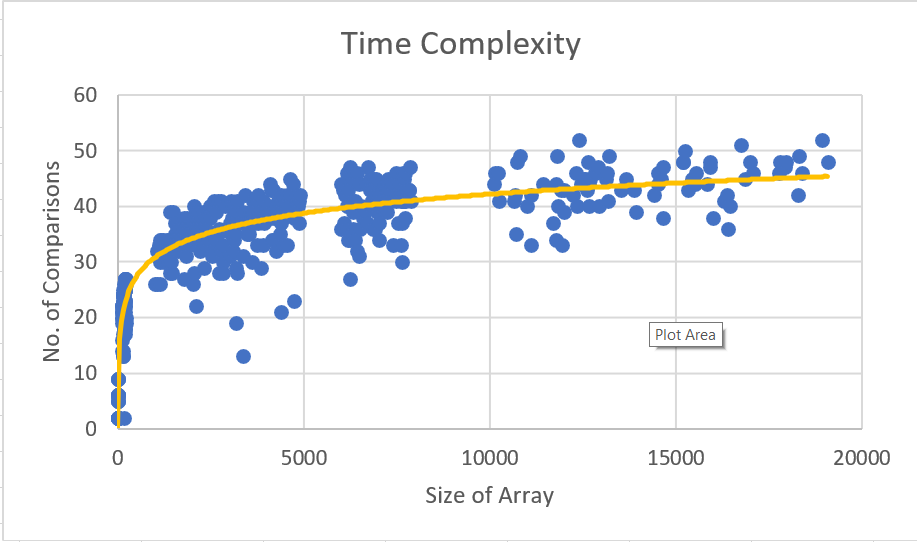
\includegraphics[width=80mm]{tc_linear.png}}
\caption{Algorithm 2 VS N Linear Scale}
\centerline{\textit{ }}
\label{fig:graph}
\end{figure}

\begin{figure}[h!]
\centerline{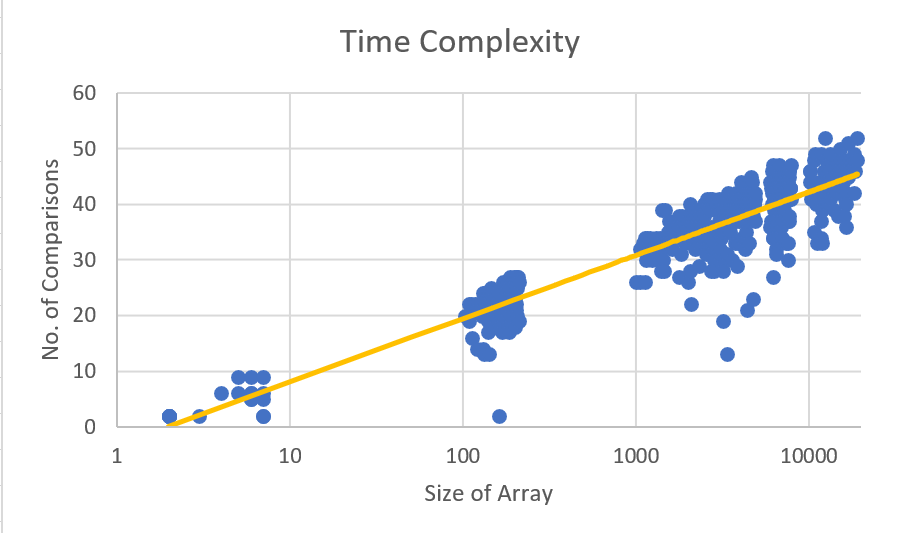
\includegraphics[width=80mm]{tc_log.png}}
\caption{Algorithm 2 VS N logarithmic Scale}
\centerline{\textit{ }}
\label{fig:graph}
 \end{figure}
\newpage

\section{Conclusion}
The more efficient algorithm, as we can see, turns out to be the 2nd algorithm (using binary search i.e. divide and conquer) against the 1st algorithm (linear search) as it has better complexity. The rotation count(pivot) will be minimum (i.e. 0) when array is already sorted.

\begin{thebibliography}{00}
\bibitem{b1}https://en.wikipedia.org/wiki/Binary\_search\_algorithm
\bibitem{b2}https://www.geeksforgeeks.org/divide-and-conquer-algorithm-introduction/
\end{thebibliography}

\end{document}
